\begin{abstract}
Relative to zero cell, native target-cell conditioning in arbitrary-scale
super-resolution improves average quality but need not improve every image
or frequency band. We diagnose
this discrepancy through fixed-checkpoint corrections, separating amplitude
overshoot from wrong-direction changes using an exact squared-error identity.
A prospective replication on 32 natural images, two model families and two
training seeds finds harmful corrections against both zero and nonzero cell
references. Relative to zero cell, native conditioning improves mean PSNR
in all four model--scale groups, yet uniform half-correction increases mean
RGB MSE by 0.26--7.55\%. Nonzero references reveal additional failures and
change which images are labelled harmful: failure is a property of a specified
correction, not an intrinsic image label. Controlled high-frequency input
paths and equal-power phase changes further produce opposite gains at fixed
scale. Together, these measurements explain why average frequency ordering,
local band damage and successful rescue of selected cases are insufficient
criteria for a globally beneficial readout correction.
\end{abstract}
\begin{keywords}
Arbitrary-scale super-resolution, cell conditioning, frequency recovery,
readout failure analysis
\end{keywords}

\section{Introduction and Related Work}
\label{sec:intro}
Arbitrary-scale super-resolution (ASISR) predicts image values at continuous
coordinates. LIIF supplies target cell size to a local decoder
\cite{chen2021liif}; LTE introduces cell-dependent phase estimation
\cite{lee2022lte}. This information specifies the requested scale but does
not guarantee that the resulting output change reduces reconstruction
error. Our question is: \emph{at the same scale and frequency band, why
can a cell-conditioned correction help one image and hurt another?}
We examine output-level failure types and controlled conditions that
change benefit, without identifying an internal neural mechanism.

Harmful cell effects are not new. LIIF already varies cell size at fixed
queries; IPE-LIIF integrates positional features and reports cases where
an additional cell input hurts \cite{liu2021ipe}. Thera supplies analytic
Gaussian filtering and discusses its mismatch with bicubic training
\cite{becker2025thera}. Our fixed-checkpoint interventions are not a
performance comparison against these methods. Integrating intermediate
features also need not equal integrating a nonlinear decoder's RGB output.

Frequency-resolved analysis has precedents in HyRA's linear/nonlinear
responses \cite{fsds2024}, texture-based error analysis
\cite{magid2022texture}, sinusoidal degradation probes
\cite{kawai2026frequency}, and Nyquist-normalised forecasting
\cite{wang2026scaleanchoring}. The importance of phase beyond spectral
magnitude is classical \cite{oppenheim1981phase}. We do not claim these
principles, or the quadratic identity below, as new. A wider continuous-SR
benchmark studies architecture and retraining effects
\cite{nasir2026empirical}; we isolate interventions on inherited models.

We study cell conditioning as an output correction with measurable
benefits and costs. The empirical contributions are: (1) paired natural-image
measurements that separate image-level from band-level harm; (2) an
overshoot/direction diagnosis, using a classical error decomposition, with
an explicit test of the cost of uniform attenuation; and (3) controlled
input-path and fixed-power phase experiments that expose conditions hidden
by coarse frequency summaries. The argument follows observed failures,
their error geometry, and interventions that change their sign.

\section{Evaluation Objects and Frequency Recovery}
\label{sec:recovery}
\subsection{Keep the comparison fixed}
Let $y=Ax$ denote the LR observation, $Q_hx$ the desired target measurement,
and $c$ the cell supplied to $F_\theta(y,q,c)$. Changes to $A$, $Q_h$ and
$c$ answer different questions. Natural-image tests use discrete HR targets
and bicubic antialiased downsampling, not certified box averages of a
known continuous field. Assigning $c=h$ does not establish that the model
implements the physical operator $Q_h$.

The LIIF/LTE/SC-INR variants inherit an EDSR-baseline encoder, DIV2K
training \cite{agustsson2017div2k}, 1000 epochs and training scales
$\times1$--$\times4$. SC-INR is the examined sinc-modulated Fourier-feature
implementation. A trained full/no-readout ablation changes weights;
a native/zero-cell comparison holds weights, observation and queries
fixed. Zero cell is outside the training cell support. Earlier probes use
one seed1 checkpoint per LTE/SC model; the new natural-image replication
uses both inherited seeds 1 and 2. The LTE snapshots omit the original
paper's extrapolation cell clamp. All interventions preserve weights.

\subsection{A useful coordinate with image-wise exceptions}
For image $i$, band $b$, target energy $S_{ib}=\|\Pi_b(x_i-\bar x_i)\|^2$
and error energy $E_{ib}=\|\Pi_b(x_i-\hat x_i)\|^2$, define
\begin{equation}
\begin{aligned}
 R_b&=1-\frac{\sum_i E_{ib}}{\sum_i S_{ib}},\\
 D&=\operatorname{median}_b[\max_s R_b(s)-\min_s R_b(s)].
\end{aligned}
 \label{eq:recovery}
\end{equation}
The frequency study uses the RGB mean, unwindowed FFTs, centre HR240
crops and respectively 14, 30 and 30 images from Set14, BSD100 and Urban100
\cite{zeyde2010single,martin2001database,huang2015urban}. With Chebyshev
frequency $\nu=\max(|\nu_x|,|\nu_y|)$ and scale $s=2,3,4$, seven bins
span $.25,.5,\ldots,2$ in $u=2s\nu$; $u=1$ is LR Nyquist. The absolute
control fixes bin edges at $\nu=u/6$. Different bin supports compare
evaluation coordinates, not equality of reconstructed functions.

Normalisation reduces $D$ in all 27 model--dataset--seed groups;
primary values fall from $.31$--$.46$ to $.013$--$.061$. This is a change
in evaluation coordinates, not a reconstruction improvement. All 24 saved-output
sensitivity settings retain the reduction. However, the original $.05$
tolerance passes only 19/27 pooled groups, versus 27/27 equal-image groups.
The repetitions share images and are not independent experiments.

Pooling can conceal the relevant variation. In Urban100, all nine pooled
curves pass $.05$, while only 14--17 of 30 images per group pass the same
descriptive tolerance. Holding image weights fixed across scales increases
$D$ in all nine Urban100 groups, although it decreases $D$ in all nine
Set14 groups. These findings motivate image-paired diagnosis: an aggregate
frequency curve cannot decide whether an individual image benefits.

\section{From Frequency Ordering to Failure Types}
\label{sec:failure}
\subsection{Coarse ordering is an insufficient explanation}
In LTE/SC seeds 2 and 3, high-band full/no-readout ablation loss
exceeds middle-band loss in 34/36 dataset--scale settings. Yet the tested
footprint score has exactly the same ranks as band index. A separate
fixed-query conditioning-average test preserves ordering in 4/4 groups,
but matches its function-similarity criterion in 0/4. Ordering alone
therefore does not establish an integral readout interpretation.
Retrained ablations and fixed-weight interventions also answer different
questions: on barbara at $\times2$, SC's high-band recovery gain is
$-.193296$ for the trained pair but $+.009733$ for native/zero cell.
We therefore hold the model fixed in the following diagnosis.

\subsection{Overshoot and wrong direction}
For fixed-weight outputs, let $F_c$ be native-cell prediction, $F_r$
a declared reference-cell prediction, $t$ the HR target, and $d=F_c-F_r$. Inner products
are pixel/channel means, optionally after band projection. Set
$a=\langle t-F_r,d\rangle$, $b=\|d\|^2$ and
\begin{equation}
 G(\lambda)=\operatorname{MSE}(F_r,t)-\operatorname{MSE}(F_r+\lambda d,t)
             =2\lambda a-\lambda^2b.
 \label{eq:gain}
\end{equation}
For a harmful native correction $G(1)<0$ and $b>0$, $0<a<b/2$ is
\emph{overshoot}: a smaller positive correction can help. When $a<0$,
the \emph{direction is wrong}: every positive multiple hurts. The oracle
optimum is $\lambda^*=a/b$. This classical identity diagnoses saved
outputs using HR truth; output interpolation is not a cell intervention
or an observation-only method. We define harm by $G(1)<-10^{-8}$. For the saved natural outputs,
$b$, $|a|$ and $|a-b/2|$ within
$64\epsilon_{64}\max(\operatorname{MSE}(F_r,t),b,10^{-8})$
are retained as numerical boundaries; $\epsilon_{64}$ is machine precision.

\subsection{Development diagnosis and prospective replication}
An initial saved-output diagnosis uses 32 development images (DIV2K
train0001--0032), centre HR128, $\times2/4$, shave4 and raw RGB.
Against zero cell, LTE has 13 harmful bands (12 overshoot, 1 wrong
 direction), and SC has 27 (14, 13). Halving the output correction rescues
11/13 and 6/27 bands, yet increases overall RGB MSE by 2.405\% and
.966\%. This motivates replication of both the failures and their
aggregate cost, rather than treating a rescued subset as a successful policy.

We freeze a new cohort, DIV2K valid0837--0868, before inference: 32 images,
LTE/SC seeds 1 and 2, and $\times2/4$. These images are separate from the
previous development and forecast evaluation cohorts and the checkpoints'
first-ten-image validation subset. The centre HR128 target and bicubic-AA
LR observation are held fixed. Each checkpoint predicts four supplied
relative cells $c_{\rm rel}=c\,n_{\rm LR}\in\{0,1/2,2/3,1\}$; native
is 1 at $\times2$ and $1/2$ at $\times4$. Training uses LR48 and integer
HR48--192, so all three nonzero values occur in the training cell's
numeric support. Changing cell at a fixed target remains mismatched
conditioning, not a joint in-distribution sample or physical target change.

All 1024 RGB predictions are hash-frozen before target scoring. The primary
contrasts are native versus zero and native versus $c_{\rm rel}=2/3$
(denoted $h3$); the other nonnative contrasts are retained. Three non-DC
Chebyshev bands use cutoffs $1/8,1/4,1/2$ on the shaved RGB channels,
with pixel-domain normalisation. Image-cluster bootstrap resamples all
32 images jointly across seeds, 10,000 times, with pointwise intervals;
repeated seeds and scales are not additional independent images.

\begin{table}[t]\centering
\caption{Prospective natural-image replication. Each row has 64 RGB and
192 band records (32 images, two seeds). RGB: all negative records
followed by those losing $>.01$ dB in parentheses. Band O/D: overshoot/
wrong-direction counts. $\Delta E_{1/2}$: half-correction mean RGB MSE
change relative to native, over all cases.}
\label{tab:failures}
\small
\begin{tabular}{lccrrr}\toprule
Model & $s$ & Ref. & RGB & Band O/D & $\Delta E_{1/2}$\\\midrule
LTE & 2 & zero & 1 (1) & 5/1 & +7.55\%\\
 & 2 & $h3$ & 13 (6) & 13/11 & +2.29\%\\
 & 4 & zero & 2 (1) & 18/2 & +2.77\%\\
 & 4 & $h3$ & 35 (10) & 21/84 & $-.058$\%\\\midrule
SC & 2 & zero & 10 (5) & 10/12 & +5.46\%\\
 & 2 & $h3$ & 17 (9) & 13/16 & +1.84\%\\
 & 4 & zero & 11 (5) & 17/30 & +.264\%\\
 & 4 & $h3$ & 25 (7) & 11/83 & +.087\%\\\bottomrule
\end{tabular}
\end{table}

\textbf{Average benefit coexists with individual harm.}
Against zero, mean native-minus-reference PSNR is $.912/.444$ dB for
LTE at $\times2/4$ and $.687/.028$ dB for SC; all four 95\% image-bootstrap
intervals are above zero. Yet Table~\ref{tab:failures} contains negative
cases in every group. The nonzero $h3$ contrast also has harmful images
in both seeds of each model and scale, so harm is not confined to zero-cell
probes. At $\times4$, 35/64 LTE and 25/64 SC RGB records are negative,
but only 10 and 7 lose more than $.01$ dB; worst losses are $.202$ and
$.136$ dB. Counts and effect sizes answer different questions.

\textbf{Failure identity depends on the correction.}
SC at $\times2$ retains all ten zero-reference negative RGB records
against $h3$. At $\times4$, its eleven zero-reference failures and
25 $h3$ failures are disjoint. Here the references lie on opposite sides
of native cell. This is a contrast change, not evidence of a new internal
mechanism. Across the two training seeds, zero-reference SC RGB harm
repeats in 10/11 image--scale cases harmed by either seed; LTE repeats in
1/2. Against $h3$, the corresponding overlaps are 17/25 and 19/29.
Failure types occur repeatedly, but exact labels and their prevalence
cannot be assigned permanently to a model or image.

\textbf{Local rescue does not imply a useful global policy.}
For the zero contrast, half-correction raises aggregate RGB MSE in all
four model--scale groups (Table~\ref{tab:failures}), with all four 95\%
intervals above zero. The same holds for $h3$ at $\times2$; at $\times4$
both intervals include zero. Thus the supported result is a repeatable
cost of this attenuation in the specified contrasts, not failure of every
possible global weight. Band losses must also be separated from RGB
losses: improvements in other bands and DC can offset a damaged band.

\begin{figure*}[t]\centering
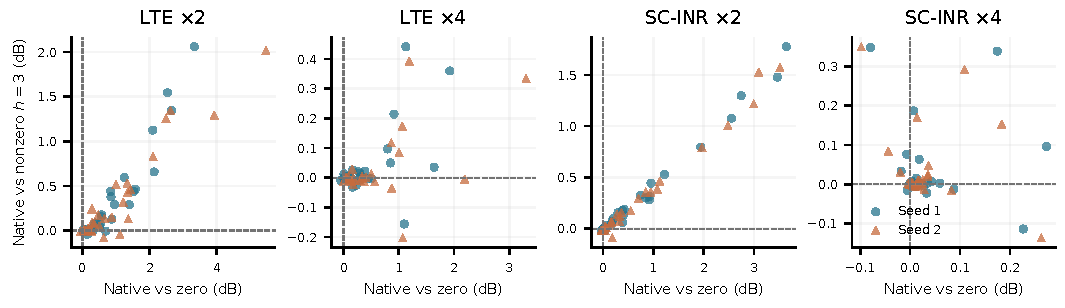
\includegraphics[width=.96\textwidth]{figures/cell-reference.pdf}
\caption{All 32 natural images under both seeds, paired at fixed model
and scale. Coordinates are full-RGB native-minus-reference PSNR gains.
Each point compares the same image under zero and nonzero $h3$ references;
negative coordinates indicate harm. Reference choice changes the harmful
subset, particularly when it changes the direction of the cell intervention.}
\label{fig:reference}
\end{figure*}

\section{Controlled Input-Path and Phase Experiments}
\label{sec:controlled}
\subsection{Design: separate two interventions}
To probe conditions behind alignment changes, we keep the two checkpoints
and $\times4$ scale fixed. A monochrome HR64 target, replicated across
RGB, is $t=.5+L+H$, with three low cosine modes
$L:\{(2,0),(0,2),(2,2)\}$ with zero initial phases. All six cosine modes
have amplitude $.04$. Frequencies are
cycles per 64 pixels. Four $H$ templates are
\begin{align*}
 M_a&=\{(10,0),(12,0),(14,0)\},\\
 M_c&=\{(10,0),(0,12),(10,10)\},\\
 H_a&=\{(18,0),(22,0),(26,0)\},\\
 H_c&=\{(18,0),(0,22),(18,18)\}.
\end{align*}
All lie above LR Nyquist (8 cycles). A low-frequency sham uses
$\{(4,0),(0,4),(4,4)\}$. Four high-branch phase vectors (one zero and
three uniform vectors, seed 20261012) are crossed with four translations
$(0,0),(.5,0),(0,.5),(.5,.5)$ in LR-pixel units. Translations move both
branches and are nested position controls, not independent mechanisms.

For each fixed target, a periodic separable bicubic-AA operator $A$
produces LR16 observations
\begin{equation}
 y_\eta=A(.5+L)+\eta A(H),\qquad \eta\in\{0,.5,1\}.
 \label{eq:path}
\end{equation}
The sham always uses $At$. Thus $\eta$ controls a specified high-frequency
input path; it also changes LR energy/gradients, not aliasing independently
of input statistics. Separately, changing high-branch phase holds each
Fourier magnitude fixed while changing the target. All modes are even,
so both full64 and primary centre32 regions contain integer periods.
No observations or outputs are clipped. Bands use the same three cutoffs
as the natural-image diagnosis, with DC excluded; gain ties use
$10^{-8}$, alignment boundaries $10^{-10}$ and tiny-change energy $10^{-12}$.
The 240 conditions contain 148
unique inputs and 296 native/zero prediction pairs, not 240 independent
images. Inputs and then all predictions were hash-frozen before scoring;
this is a deterministic diagnostic, not a blinded natural-image test.



\subsection{Alignment reversals and fixed-power counterexamples}
For the two middle-frequency templates (32 phase--position conditions),
increasing $\eta$ from 0 to 1 lowers middle-band gain in 29/32 LTE and
32/32 SC conditions. Harmful outcomes increase from 18 to 32 and 15 to
31, respectively; 14/32 and 16/32 change from positive to negative
alignment $a$. Full64 evaluation retains gain decreases in 31/32 for
both models, although exact negative counts change. The high-frequency
templates instead contain both signs of path effect
across the fixed grid; the path is not uniformly harmful.

At $\eta=1$, changing phase at fixed template and position produces both
positive and negative high-band gains in all eight template--position
groups per model, in both evaluation regions. Thus \emph{target power
alone does not determine readout benefit in these fixed models}.
This does not hold LR power/gradients fixed. At $\eta=0$, high-phase
variants share identical inputs and outputs: score differences then
reflect different unobserved targets, not a neural response to hidden
phase. These distinctions prevent phase sensitivity from being mistaken
for a general adaptive mechanism.

Effects are small: at $\eta=1$ in the high templates, centre-region
full-RGB native-minus-zero PSNR spans $[-.00730,.01236]$ dB for LTE and
$[-.00164,.000891]$ dB for SC. Sign reversals provide diagnostic
counterexamples, not a practical performance advance or an estimate
of natural-image causal prevalence.

\section{Guidance, Scope and Conclusion}
\label{sec:limits}
\textbf{Explanation does not yet supply a selector.}
For bicubic upsampling $B(y)$, the observable proxy replaces $t$ in
Eq.~\eqref{eq:gain}; true gain minus proxy gain is exactly
$2\langle t-B(y),d\rangle$. Unlike generalized SURE under its stated
assumptions \cite{eldar2008gsure}, this proxy has no unbiased-risk guarantee.
With 32 calibration and 12 separate evaluation images (valid0825--0836),
forecasts were frozen before scoring. SC's magnitude/spectrum ridge
detects 6/14 harmful bands with 15 false positives; adding proxy alignment
still detects six with 17 false positives (balanced accuracy $.585$
versus $.568$). Neither candidate establishes a reliable RGB policy gain;
LTE has only one harmful band outcome. Saved-output crop/band sensitivity
retains SC harm without repairing the forecasts.

A second, retrospective test uses lower-resolution reconstruction gains
with eight-fold whole-image-held-out fitting on the 32 development images.
Both paired image-bootstrap AUC improvements include zero. Directly
selecting native/zero by the lower-level gain increases RGB MSE by
$.239\%$ (LTE) and $.142\%$ (SC). Thus neither tested proxy provides a
reliable operational substitute for the HR-assisted diagnosis. 

\textbf{Scope and cost.}
The strongest natural-image evidence concerns the declared output
contrasts on two model families and two training seeds. Synthetic periodicity
and a finite phase grid limit the controlled examples; they do not identify
the causal prevalence of aliasing in natural images. The zero reference
is unsupported, while the nonzero controls establish numeric cell support
only. No matching training or new architecture is introduced. Independent
pixel/FFT and bootstrap recomputation verifies saved scoring, rather than
reimplementing the networks. The new complete experiment takes 637.27
seconds on one CPU thread, with 6.88 seconds for independent audit and no
GPU; excluded-image preflight inference/scoring takes 27.28 seconds, followed
by a $.17$-second scoring repair. The original failed serialization is retained.
The earlier controlled experiment takes 85.32 seconds on one CPU thread.

\textbf{Conclusion.}
Relative to zero cell, native conditioning improves average reconstruction
in the tested models,
while individual corrections can overshoot or move away from the target.
The new natural-image replication establishes failures against nonzero
references and across training seeds, while showing that their identities
remain contrast-dependent. Controlled input paths and fixed-power phase
changes expose structure omitted by band-energy summaries. A useful
assessment of readout must therefore report the specified correction,
its failure type, the actual image-level loss, and the aggregate cost of
any proposed rescue. The present evidence supports this diagnostic
framework; a reliable observation-only correction rule remains open.

\section{Acknowledgments}
Claude and OpenAI Codex assisted with text, analysis code, figures and
record checks. Numerical records were audited; human author review and
responsibility are required before submission.
